\documentclass[conference]{IEEEtran}
\IEEEoverridecommandlockouts
\usepackage[utf8]{inputenc}
\usepackage[T1]{fontenc}
\usepackage[brazil]{babel}
\usepackage{cite}
\usepackage{amsmath,amssymb}
\usepackage{algorithm}
\usepackage[noend]{algpseudocode}
\usepackage{graphicx}
\usepackage{booktabs}
\usepackage{multirow}
\usepackage{xcolor}
\usepackage{url}
\usepackage[hidelinks]{hyperref}
\graphicspath{{figs/}}
\floatname{algorithm}{Algoritmo}
\renewcommand{\algorithmicrequire}{\textbf{Entrada:}}
\renewcommand{\algorithmicensure}{\textbf{Saída:}}
\newcommand{\modus}{\textsc{Modus}}
\newcommand{\modusp}{\textsc{Modus}++}

\begin{document}

\title{Replicação e Extensão do \modus: Vazamento de Rótulo, Envenenamento por \emph{Flood} e
Defesas para Detecção Online Não Supervisionada de DDoS}

\author{
\IEEEauthorblockN{Pedro Henrique, Rodrigo Amaral, Emanuell da Luz}
\IEEEauthorblockA{Centro de Informática (CIn) -- Universidade Federal de Pernambuco (UFPE)\\
Recife, PE, Brasil}
}

\maketitle

\begin{abstract}
O \modus\ é um detector online e não supervisionado de DDoS que combina ADWIN, Half-Space Trees
(HST) e um limiar robusto, com F1 reportado de até 99,62\%. Este trabalho replica o método a partir
do texto do artigo, em três bases públicas, e implementa as melhorias propostas na primeira etapa
da replicação. Ao reescrever o HST, encontramos um vazamento de rótulo: o \texttt{HSTrees} do MOA
conta o atributo de classe como dimensão de corte. Com o rótulo no fluxo, reproduzimos os 99,62\%
do ASEADOS-SDN-IoT (obtivemos 99,73\%); sem ele, o F1 cai para 0,00\%. Sem o vazamento aparece o
problema real: o \emph{flood} entra no treino seletivo e vira o perfil normal, com 99,96\% a
100\% do ataque usado no treino. Propomos o \modusp, que soma a uma versão normalizada do método
quatro defesas, todas causais e sem rótulos: janela de referência em tempo, aquecimento adaptativo,
teto de treino por destino e um modelo de referência congelado. Com uma única configuração, fixada
antes das rodadas, o F1 sobe de 0,08\% para 62,99\% no ASEADOS e de 76,66\% para 91,17\% no
Edge-IIoTset com 14 tipos de ataque. No CTU-13 o envenenamento cai de 100\% para 2,41\%, mas o F1
a priori fica em 0,01\%: o \emph{flood} pontua logo abaixo do limiar congelado. A calibração do
limiar sem rótulos é a limitação que permanece.
\end{abstract}

\begin{IEEEkeywords}
DDoS, detecção de anomalias, fluxos de dados, Half-Space Trees, envenenamento, vazamento de rótulo,
reprodutibilidade
\end{IEEEkeywords}

\section{Introdução}
\label{sec:intro}

Ataques distribuídos de negação de serviço (DDoS) continuam entre as ameaças mais frequentes à
disponibilidade de serviços em rede, e os relatórios de operadoras de mitigação registram novos
vetores a cada trimestre~\cite{cloudflare2026}. Detectores supervisionados dependem de tráfego
rotulado, que envelhece rápido e não cobre vetores novos. Por isso há interesse em detectores
\emph{online} e \emph{não supervisionados}, que aprendem o perfil do tráfego legítimo durante a
operação e apontam o que foge dele~\cite{mirsky2018kitsune}. Métodos de isolamento, como o
Isolation Forest~\cite{liu2008iforest} e sua variante para fluxos, as Half-Space
Trees~\cite{tan2011hst}, são a base usual desses detectores, pois têm custo constante por instância.

O \modus~\cite{modus2026}, publicado no SBSeg 2026, segue essa linha. O método combina um detector
de mudança de conceito (ADWIN), um HST e um limiar baseado em mediana e MAD, e reporta F1 de
99,62\%, 83,79\% e 81,24\% em três bases públicas. O código dos autores não está disponível. Este
artigo relata uma replicação independente, feita em duas etapas na disciplina de Auditoria e
Segurança de Sistemas de Informação do CIn/UFPE.

Na Etapa~1 reimplementamos o método a partir do texto e comparamos os resultados com os do artigo.
Dois dos três números se reproduziram, e a análise apontou fragilidades: a \emph{flag} de mudança
de conceito não altera as predições, o HST sem normalização separa por protocolo e não por volume,
e o limiar depende de um piso ajustado por base. A etapa terminou com quatro melhorias propostas e
três defesas indicadas como trabalho futuro.

Na Etapa~2, objeto principal deste artigo, implementamos as melhorias. Para controlar a janela de
referência do HST, reescrevemos o algoritmo em \texttt{numpy}, bit a bit igual ao do MOA. A
reescrita revelou um defeito que muda a leitura da Etapa~1: o \texttt{HSTrees} do MOA inclui o
atributo de classe entre as dimensões de corte. Quando o fluxo carrega o rótulo verdadeiro, o
detector ``não supervisionado'' usa o rótulo. A réplica dos 99,62\% no ASEADOS-SDN-IoT só existe
com esse vazamento.

Removido o vazamento, o detector falha por outro motivo, mais geral. O treino seletivo, que só
aprende com o que foi predito como benigno, não protege o modelo: basta o início do ataque passar
pelo limiar para que o \emph{flood}, por ser denso, domine a massa do HST e vire o perfil de
referência. A partir daí o ataque é o tráfego \emph{mais normal} do fluxo.

\subsection*{Contribuições}
\begin{itemize}
\item \textbf{Replicação independente} do \modus\ nas três bases do artigo, com a reconstrução
exata do número de instâncias de cada uma e a identificação de inconsistências nos rótulos do
CTU-13 e na composição do Edge-IIoTset (Seção~\ref{sec:replication}).
\item \textbf{Vazamento de rótulo no \texttt{HSTrees} do MOA}: descrição do mecanismo, teste direto
e medição do efeito por base. No ASEADOS o F1 vai de 99,73\% para 0,00\% (Seção~\ref{sec:leak}).
\item \textbf{HST em \texttt{numpy} equivalente ao do MOA}, com diferença máxima de
$2{,}2\times10^{-16}$ nos scores, sem a dimensão do rótulo e com controle da janela de referência
(Seção~\ref{sec:hstnp}).
\item \textbf{Medição do envenenamento por \emph{flood}}: a fração do ataque usada no treino do
modelo, reportada em todas as rodadas (Seção~\ref{sec:results}).
\item \textbf{\modusp}: quatro defesas causais e sem rótulos, avaliadas com uma única configuração
fixada a priori, com ablação, sementes e sensibilidade (Seções~\ref{sec:method}
e~\ref{sec:results}).
\end{itemize}

Os resultados são mistos, e os reportamos assim. O \modusp\ leva o F1 de 0,08\% para 62,99\% no
ASEADOS e de 76,66\% para 91,17\% no Edge-IIoTset com 14 tipos de ataque. No CTU-13 o
envenenamento praticamente desaparece, mas o F1 a priori fica em 0,01\%, porque o score do
\emph{flood} fica milésimos abaixo do limiar. Todos os números deste artigo vêm de rodadas salvas
no repositório do trabalho, com configuração, \emph{log} e métricas.

O restante do texto está organizado assim. A Seção~\ref{sec:background} apresenta os fundamentos e
o \modus. A Seção~\ref{sec:replication} resume a replicação e descreve o vazamento. A
Seção~\ref{sec:method} detalha o \modusp, e a Seção~\ref{sec:setup}, a metodologia. A
Seção~\ref{sec:results} traz os resultados, a Seção~\ref{sec:discussion} os discute, e a
Seção~\ref{sec:conclusion} conclui.

\section{Fundamentação e Trabalhos Relacionados}
\label{sec:background}

\subsection{Detecção de anomalias em fluxos}
No paradigma de fluxo de dados, cada instância é processada uma única vez, na ordem de chegada,
com memória limitada e sem acesso ao futuro~\cite{gama2014drift}. A avaliação usual é
\emph{test-then-train}: o modelo pontua a instância e só então pode aprender com ela. Para tráfego
de rede, a vantagem é dupla: o detector acompanha a deriva do tráfego legítimo e não exige rótulos,
o que em tese permite detectar ataques nunca vistos~\cite{mirsky2018kitsune}. O preço é conhecido:
um detector que aprende continuamente com o tráfego também pode aprender o ataque.

\subsection{Half-Space Trees}
As Half-Space Trees (HST)~\cite{tan2011hst} são um conjunto de árvores binárias completas,
construídas \emph{sem olhar os dados}: cada nó corta um atributo sorteado no ponto médio do seu
espaço de trabalho, que é um intervalo aleatório em torno de $[0,1]$. Por isso o HST pressupõe
atributos normalizados nesse intervalo. Cada nó guarda duas massas: $r$, a contagem de instâncias da
janela de referência (a anterior), e $l$, a da janela corrente. O score de uma instância soma, em
cada árvore, $r \cdot 2^{p}$ no primeiro nó do seu caminho com massa abaixo de um limite
(\emph{size limit}), onde $p$ é a profundidade desse nó. Pouca massa em regiões rasas indica
anomalia. Ao fim de cada janela de $W$ instâncias, $r \leftarrow l$ e $l \leftarrow 0$. No MOA~\cite{bifet2010moa},
usado pelo CapyMOA~\cite{gomes2025capymoa}, o score é normalizado para $[0,1]$ com $1$ = anômalo.

\subsection{ADWIN e limiar robusto}
O ADWIN~\cite{bifet2007adwin} mantém uma janela de tamanho variável sobre uma sequência numérica e
corta a parte antiga quando duas subjanelas têm médias estatisticamente diferentes (parâmetro
$\delta$). É o detector de mudança de conceito mais usado em fluxos. Para limiares sobre scores, o
\modus\ usa mediana e desvio absoluto mediano (MAD), robustos a valores extremos. O critério do
z-score modificado de Iglewicz e Hoaglin~\cite{iglewicz1993outliers} marca como \emph{outlier} um
valor com $0{,}6745\,(s-\tilde{s})/\mathrm{MAD} > 3{,}5$, ou seja, $s > \tilde{s} + 5{,}19\cdot\mathrm{MAD}$.

\subsection{Envenenamento de detectores de anomalia}
Detectores que se retreinam com o tráfego observado são vulneráveis a envenenamento: o atacante
desloca gradualmente o perfil ``normal'' até que o ataque passe despercebido. O ANTIDOTE~\cite{rubinstein2009antidote}
mostrou isso para detectores baseados em PCA e propôs estimadores robustos como defesa. Em DDoS
volumétrico nem é preciso um atacante sofisticado: o próprio \emph{flood} é tão denso que, se
uma fração dele entra no treino, passa a dominar a massa do modelo. A defesa comum dos
detectores online é treinar só com o que foi predito como benigno~\cite{modus2026}; mostramos
na Seção~\ref{sec:results} que isso não basta.

\subsection{Armadilhas metodológicas}
Arp \emph{et al.}~\cite{arp2022dos} catalogam erros recorrentes de aprendizado de máquina em
segurança. Três deles aparecem neste trabalho: \emph{data snooping} (normalização com estatísticas
do conjunto inteiro), \emph{label leakage}~\cite{kaufman2012leakage} (informação do rótulo chegando
ao modelo) e ajuste de hiperparâmetros por base de teste. Sommer e Paxson~\cite{sommer2010outside}
já alertavam que detectores de anomalia em redes tendem a acertar pelos motivos errados quando a
avaliação não isola o que o modelo realmente aprendeu. Replicações independentes são o principal
remédio para esses problemas~\cite{baker2016reproducibility}.

\subsection{O método \modus}
O \modus~\cite{modus2026} propõe três fases aplicadas a cada pacote (ou fluxo):
(a) preparação: ordenação temporal, seleção de quatro atributos (portas de origem e destino,
protocolo e tamanho) e vetorização;
(b) mudança de conceito: um ADWIN monitora o tamanho do pacote e emite uma \emph{flag} binária,
concatenada ao vetor como quinto atributo;
(c) detecção: um HST pontua a instância, que é ataque se o score passa do limiar
$\tau = \min(\tau_{\max}, \max(\tau_{\min}, \tilde{S} + \alpha\cdot\mathrm{MAD}(S)))$, calculado
sobre uma janela $S$ de scores recentes. Após um aquecimento de $B=50.000$ instâncias, só as
instâncias preditas como benignas treinam o HST e entram em $S$. A contribuição central alegada é
usar a mudança de conceito como \emph{informação} para o detector, e não só como gatilho de
retreino. O artigo reporta F1 de 99,62\% (ASEADOS-SDN-IoT~\cite{aseados}), 83,79\%
(CTU-13, cenário 11~\cite{garcia2014ctu13}) e 81,24\% (Edge-IIoTset~\cite{ferrag2022edgeiiot}),
com hiperparâmetros ($W$, nº de árvores, profundidade, $\alpha$, $\tau_{\min}$, $\tau_{\max}$)
escolhidos por base.

\section{Replicação do \modus\ (Etapa 1) e Vazamento de Rótulo}
\label{sec:replication}

Não há código público dos autores. Reimplementamos o \modus\ a partir do texto, em Python, com o
HST e o ADWIN do CapyMOA~\cite{gomes2025capymoa}, que encapsula o MOA~\cite{bifet2010moa}. Os
hiperparâmetros são os da Seção~4.1 do artigo, por base. Nas três bases chegamos exatamente ao
número de instâncias reportado. No ASEADOS são 312.262 fluxos (classes Benign e DDoS). No CTU-13
são 6.336.394 pacotes IPv4 do \emph{pcap} truncado do cenário 11. No Edge-IIoTset são 30.919.961
quadros: a única combinação que fecha esse total usa os \emph{pcaps} normais duas vezes, o
\emph{Port Scanning} como benigno e os quatro DDoS.

\subsection{Resultados da Etapa 1}
A Tabela~\ref{tab:repl} resume a replicação. No ASEADOS e no Edge-IIoT os números do artigo se
reproduzem; no Edge-IIoT, os verdadeiros positivos e falsos negativos são idênticos pacote a pacote.
No CTU-13 a replicação não fecha: os rótulos do artigo são internamente inconsistentes. A regra
oficial do CTU-13 (IPs infectados) dá 32,04\% de ataques, exatamente o valor que a Tabela~1 do
artigo chama de ``Benigno'', e a matriz de confusão implica 2,89 milhões de ataques, total que
nenhuma regra testada reproduz. A análise da Etapa~1 mostrou ainda que:
(i) a \emph{flag} do ADWIN, contribuição central do artigo, não altera nenhuma predição no CTU-13 e
altera um pacote em 19,6 milhões no Edge-IIoT;
(ii) sem normalização, o HST separa por protocolo e não por volume: os cortes caem em $[0,1]$ e
portas e tamanhos ficam sempre do mesmo lado. O recall de 73,16\% no Edge-IIoT é exatamente a
fração de DDoS que não é TCP;
(iii) o limiar passa quase todo o tempo preso no piso $\tau_{\min}$, ajustado à mão por base;
(iv) no ASEADOS, a ordem ``temporal'' que reproduz o artigo vem de um erro de leitura de datas
(dd/mm lido como mm/dd). Na ordem cronológica correta o DDoS ocorre durante o aquecimento e o F1 é 0\%.

\begin{table}[t]
\centering
\caption{Replicação do \modus\ (F1 \%, convenção do artigo). ``Com rótulo'': o HST do MOA recebe o
rótulo verdadeiro como atributo (Etapa~1). ``Sem rótulo'': fluxo corrigido. $^{*}$Medido no conjunto
sem a duplicação do tráfego normal (19,6 milhões de quadros), no qual a rodada com rótulo também dá 84,42.}
\label{tab:repl}
\begin{tabular}{lccc}
\toprule
Base & Artigo & Com rótulo & Sem rótulo \\
\midrule
ASEADOS-SDN-IoT & 99,62 & 99,73 & \textbf{0,00} \\
CTU-13 (C11)    & 83,79 & 64,55 & 64,55 \\
Edge-IIoTset    & 81,24 & 84,33 & 84,42$^{*}$ \\
\bottomrule
\end{tabular}
\end{table}

\subsection{O HSTrees do MOA usa o rótulo como atributo}
\label{sec:leak}
Ao portar o HST para \texttt{numpy} (Seção~\ref{sec:hstnp}), notamos que o MOA dimensiona o espaço de
trabalho com \texttt{instance.numAttributes()}, que \emph{inclui o atributo de classe}. Quando o fluxo
carrega o rótulo verdadeiro, como no uso padrão do CapyMOA, em que \texttt{NumpyStream} recebe
\texttt{X} e \texttt{y}, cerca de $1/(d+1)$ dos cortes de cada árvore separam ataque de benigno pelo
próprio rótulo. Isso também vale para a pontuação, porque \texttt{score\_instance} recebe a mesma
instância. Verificamos o efeito diretamente: com o mesmo vetor de atributos e só o rótulo trocado,
o score do MOA muda até 0,10.

O efeito sobre a replicação depende de os atributos já separarem as classes. No CTU-13 eles
separam: o \emph{flood} é ICMP. As predições com e sem rótulo são idênticas nas 6,3 milhões de
instâncias. No ASEADOS não separam: todo fluxo DDoS é o vetor $[0,0,0,0]$, idêntico a 42.740 fluxos
benignos, e o que dava a esses fluxos o score constante de 0,806, acima do piso de 0,75, era a
dimensão do rótulo. Sem ela, o recall cai de 100\% para 0\% e a AUC-ROC de 1,00 para 0,11. O
detector passa a considerar o DDoS \emph{mais normal} que o tráfego benigno: o ataque passa no
início, treina o modelo e vira o perfil de referência.

Não sabemos se a implementação dos autores tem o mesmo problema, pois o código não é público. O
resultado mostra, porém, que os 99,62\% no
ASEADOS são reproduzíveis \emph{exatamente} com o vazamento e não são reproduzíveis sem ele. Daqui
em diante, todas as rodadas usam o fluxo corrigido: o MOA recebe um rótulo constante, e o motor
\texttt{numpy} não tem a dimensão do rótulo.

\section{\modusp: Melhorias Implementadas}
\label{sec:method}

A Etapa~1 propôs quatro melhorias: normalização online, atributos de taxa por janela, aquecimento
adaptativo e teste com ataques não-DDoS. As duas primeiras formam o que chamamos de \modus+.
Elas já haviam sido implementadas e avaliadas, mas com o vazamento de rótulo descrito na
Seção~\ref{sec:replication}. A Etapa~1 também identificou o envenenamento por \emph{flood} como
limitação estrutural e apontou três defesas como trabalho futuro. Nesta etapa implementamos o
aquecimento adaptativo e as três defesas, e reavaliamos tudo sem vazamento. O conjunto resultante é
o \modusp. Cada componente é independente e pode ser ligado por uma opção da linha de comando, o
que permite a ablação da Seção~\ref{sec:results}.

\subsection{HST sem vazamento, com controle da janela}
\label{sec:hstnp}
O HSTrees do MOA só troca a janela de referência por contagem de instâncias treinadas, normaliza o
score pelo tamanho nominal $W$ e não expõe as massas. Reimplementamos o HST em
\texttt{numpy}, fiel ao MOA:
(i) o gerador \texttt{java.util.Random} reproduzido bit a bit, com a mesma ordem de sorteios;
(ii) o mesmo espaço de trabalho por dimensão, $[s-2\max(s,1-s),\, s+2\max(s,1-s)]$ com
$s\sim U[0,1]$;
(iii) um detalhe do MOA que não está no artigo original do HST: os vetores de mínimo e máximo do
espaço de trabalho são compartilhados entre os nós, e o construtor restaura o máximo após criar o
filho esquerdo, mas não restaura o mínimo após o direito;
(iv) a mesma fase inicial, em que as primeiras 51 instâncias entram direto na referência e o score
vale 0,5.
Um script de validação compara os scores com os do MOA, instância a instância, em três
configurações; a maior diferença é $2{,}2\times10^{-16}$. Com uma dimensão constante no lugar do
rótulo, o motor novo reproduz exatamente as predições do MOA sem rótulo. A vantagem prática é que
o score de uma janela inteira pode ser calculado em lote, pois a referência $r$ não muda entre
trocas; só a decisão de treinar é sequencial. Nas rodadas do \modusp\ a dimensão do rótulo é
simplesmente omitida.

\subsection{Atributos e normalização (\modus+)}
Os quatro atributos do artigo recebem $\log(1+x)$ no tamanho e Min-Max \emph{causal}: cada coluna
é escalada pelo mínimo e máximo observados até a instância atual, o que elimina o
\emph{data snooping} do Min-Max global. Somam-se duas taxas: pacotes por segundo no último segundo,
global e por IP de destino, ambas com $\log(1+x)$. A taxa dá ao detector a noção de \emph{volume},
que é o que caracteriza um DDoS e que os quatro atributos originais não capturam.

O Min-Max causal tem um efeito colateral: um \emph{flood} com taxa inédita estica o máximo da
coluna e comprime todo o tráfego normal para perto de zero. A opção de \textbf{normalização
congelada} fixa mínimo e máximo ao fim das $B$ primeiras instâncias. Depois disso, valores fora do
intervalo ficam fora de $[0,1]$, o que o HST suporta, pois seu espaço de trabalho vai de cerca de
$-1$ a $2$.

\subsection{Melhoria 1: janela de referência em tempo}
No HST original a referência é trocada a cada $W$ instâncias treinadas. Num \emph{flood} de 17 mil
pacotes/s e $W=250$, isso dá 70 trocas por segundo: basta uma fração do ataque passar pelo limiar
para que, em milissegundos, a referência seja feita só de ataque. No \modusp\ a referência é trocada
a cada $T$ segundos do relógio do fluxo (adotamos $T=10$\,s a priori). A troca só ocorre se a janela
que termina tiver ao menos 50 instâncias treinadas; caso contrário, ela continua acumulando. A
normalização do score passa a usar a massa real da referência, e não um $W$ nominal. Assim o ritmo
de adaptação do modelo deixa de ser ditado pela taxa de chegada, que é justamente o que o atacante
controla.

\subsection{Melhoria 2: aquecimento adaptativo}
O \modus\ treina às cegas nas $B=50.000$ primeiras instâncias, um número que corresponde a 15\,s no
CTU-13 e a quatro dias no ASEADOS. No \modusp\ um ADWIN ($\delta=0{,}002$) monitora o score do HST
durante o aquecimento. O aquecimento termina na primeira instância $t \geq B_{\min}$ que esteja
$B_{\mathrm{est}}$ instâncias sem mudança detectada, com teto em $B_{\max}$. Usamos
$B_{\min}=B_{\mathrm{est}}=5.000$ e $B_{\max}=50.000$, o valor do artigo. O critério não usa rótulos.

\subsection{Melhoria 3: teto de treino por intervalo}
Treinar só o que foi predito como benigno não limita \emph{quanto} se treina. No \modusp, a cada
segundo, no máximo $c$ instâncias por IP de destino podem treinar o modelo e entrar na janela $S$
do limiar. As demais são pontuadas e classificadas normalmente, mas descartadas do treino. O teto
$c$ é o percentil 99 das contagens por (segundo, destino) observadas no aquecimento, sem rótulos.
Um \emph{flood} contra um alvo contribui no máximo com $c$ instâncias por segundo, por mais
intenso que seja.

\subsection{Melhoria 4: modelo de referência congelado}
Ao fim do aquecimento, um segundo HST (outra semente) é construído com os primeiros 80\% do
aquecimento e nunca mais é atualizado. Seu limiar $\tau_f$ é o quantil 0,999 dos seus scores nos
20\% finais do aquecimento, que ele não viu. Uma instância é ataque se o modelo adaptativo
\emph{ou} o congelado disparar, e só treina o modelo adaptativo se nenhum dos dois disparar.
O modelo congelado é a âncora que não pode ser envenenada. O adaptativo continua acompanhando a
deriva legítima, mas não consegue mais ``aprender'' um ataque que o congelado ainda reconhece como
anômalo. O custo esperado é mais falsos positivos quando o tráfego legítimo muda muito em relação
ao aquecimento.

\begin{algorithm}[t]
\caption{Laço do \modusp\ (por instância $x_t$, no instante $\mathit{ts}_t$)}
\label{alg:modusp}
\begin{algorithmic}[1]
\small
\Require HST adaptativo $H$, janela $T$, teto $c$, HST congelado $F$ e limiar $\tau_f$ (após o aquecimento)
\If{$\lfloor \mathit{ts}_t/T \rfloor$ mudou \textbf{e} $|l_H| \geq 50$} \State $H.r \gets H.l$; $H.l \gets 0$ \EndIf
\State $s \gets H.\mathrm{score}(x_t)$;\ $s_f \gets F.\mathrm{score}(x_t)$
\If{aquecendo} \State treina $H$; $S \gets S \cup \{s\}$; atualiza ADWIN com $s$
  \If{$t\geq B_{\min}$ e ADWIN estável há $B_{\mathrm{est}}$ (ou $t = B_{\max}$)} \State fim do aquecimento: calcula $c$, constrói $F$ e $\tau_f$ \EndIf
\Else
  \State $\tau \gets \max(\tau_{\min}, \tilde{S} + \alpha\,\mathrm{MAD}(S))$
  \If{$s > \tau$ \textbf{ou} $s_f > \tau_f$} \State \textbf{alarme} \Comment{não treina}
  \ElsIf{treinos de $\mathrm{dst}(x_t)$ neste segundo $< c$} \State treina $H$ com $x_t$; $S \gets S \cup \{s\}$
  \EndIf
\EndIf
\end{algorithmic}
\end{algorithm}

O Algoritmo~\ref{alg:modusp} resume o laço. Todas as decisões em $t$ dependem só de
$x_1,\dots,x_t$: o método continua de passagem única e causal. As opções são independentes; com
todas desligadas, o laço é o do \modus.

\section{Metodologia Experimental}
\label{sec:setup}

\subsection{Bases}
\textbf{ASEADOS-SDN-IoT}~\cite{aseados}: registros de fluxo de uma rede SDN-IoT. Usamos as classes
Benign e DDoS (312.262 fluxos, 16,5\% de ataque), como o artigo, e todas as cinco classes (Benign,
Bot, DDoS, DoS, Probe; 457.044 fluxos) para o teste com ataques não-DDoS. A ordem é a do artigo
(Seção~\ref{sec:replication}), em que o DDoS dura 1.117\,s, a cerca de 46 fluxos/s, depois de
233 mil fluxos benignos.
\textbf{CTU-13, cenário 11}~\cite{garcia2014ctu13}: 6.336.394 pacotes em 971\,s (cerca de
6.500 pacotes/s), com o \emph{botnet} Rbot fazendo um \emph{flood} ICMP de cerca de 17 mil
pacotes/s contra um alvo. O rótulo é a regra oficial: o pacote é ataque se envolve um dos três IPs
infectados (32,0\%).
\textbf{Edge-IIoTset}~\cite{ferrag2022edgeiiot}: \emph{pcaps} de um \emph{testbed} IIoT, todos os
quadros, ordenados por tempo.

\subsection{Configurações}
Para não ajustar hiperparâmetros na base de teste, todas as rodadas do \modusp\ usam uma única
configuração, \texttt{fixed\_q}, definida na Etapa~1:
HST com os valores padrão de Tan \emph{et al.}~\cite{tan2011hst} ($W=250$, 25 árvores, profundidade
15, \emph{size limit} 0,1); limiar $\tilde{S} + 5{,}19\cdot\mathrm{MAD}$ (z-score modificado de
Iglewicz e Hoaglin) sobre $|S|=5.000$; piso automático igual ao quantil 0,999 dos scores do
aquecimento; e ADWIN com $\delta=0{,}001$ no tamanho. Os parâmetros novos foram fixados antes das
rodadas: janela de 10\,s, teto por destino no percentil 99 do aquecimento, quantil 0,999 para o
limiar congelado, $B_{\min}=B_{\mathrm{est}}=5.000$ e $B_{\max}=50.000$. As variações desses
valores aparecem apenas como análise de sensibilidade (Seção~\ref{sec:sens}), sempre identificadas
como tal. Como referência, reportamos também o \modus\ com os hiperparâmetros do artigo para cada
base.

\subsection{Métricas}
Reportamos precisão, recall e F1 da classe ataque na fase operacional, isto é, após o fim do
aquecimento de cada rodada. Para comparar aquecimentos de tamanhos diferentes, também calculamos as
métricas no trecho comum após as 50 mil instâncias. Reportamos ainda duas métricas independentes
de limiar: a AUC-ROC e a PR-AUC dos scores (no \modusp, do modelo adaptativo; quando indicado, do
congelado). Para medir o envenenamento diretamente, reportamos a fração das instâncias de ataque
pós-aquecimento que foram usadas no treino do modelo adaptativo.

\subsection{Implementação e reprodutibilidade}
O código, os \emph{logs} e as métricas de todas as rodadas estão no repositório do trabalho. Os
\emph{scores} por instância são regenerados pelo \texttt{run.py}. As rodadas foram feitas em um Mac
ARM de 10 núcleos e 16\,GB, com Python 3.13, CapyMOA 0.15 e OpenJDK 17, várias em paralelo. Por isso
os tempos são indicativos.

\section{Resultados}
\label{sec:results}

Todos os números desta seção são da fase operacional, sem rótulo no fluxo. A
Tabela~\ref{tab:main} reúne as rodadas principais. ``Env.'' é a fração das instâncias de ataque
pós-aquecimento usadas no treino do modelo adaptativo. O motor MOA não registra essa fração.

\begin{table}[t]
\centering
\caption{Resultados sem vazamento, fase operacional (\%). \modus: hiperparâmetros do artigo para a
base. \modus+ e \modusp: configuração única \texttt{fixed\_q}.}
\label{tab:main}
\setlength{\tabcolsep}{2.6pt}
\begin{tabular}{llrrrrr}
\toprule
Base & Método & Prec. & Rec. & F1 & FPR & Env. \\
\midrule
\multirow{3}{*}{\shortstack[l]{ASEADOS\\(DDoS)}}
 & \modus    &  0,00 &  0,00 &  0,00 &  0,13 & -- \\
 & \modus+   &  0,43 &  0,04 &  0,08 &  2,39 & 99,96 \\
 & \modusp   & 95,19 & 47,07 & \textbf{62,99} &  0,48 & 51,24 \\
\midrule
\multirow{3}{*}{\shortstack[l]{ASEADOS\\(5 classes)}}
 & \modus    &  0,00 &  0,00 &  0,00 &  0,00 & -- \\
 & \modus+   & 77,78 &  0,35 &  0,71 &  0,08 & 99,65 \\
 & \modusp   & 47,83 & 23,09 & \textbf{31,15} & 17,88 & 66,02 \\
\midrule
\multirow{4}{*}{\shortstack[l]{CTU-13\\(C11)}}
 & \modus    & 47,66 & 99,97 & 64,55 & 52,37 & -- \\
 & \modus+   &  0,01 &  0,00 &  0,00 &  3,12 & 100,00 \\
 & \modus+ e congelado & 90,79 & 56,42 & \textbf{69,59} & 2,73 & 43,58 \\
 & \modusp   &  0,06 &  0,00 &  0,01 &  2,60 & 2,41 \\
\midrule
\multirow{3}{*}{\shortstack[l]{Edge-IIoT\\(14 ataques)}}
 & \modus    & 99,79 & 62,23 & 76,66 &  0,12 & -- \\
 & \modus+   & 43,95 &  0,01 &  0,01 &  0,01 & 99,99 \\
 & \modusp   & 96,03 & 86,77 & \textbf{91,17} &  3,14 & 6,90 \\
\bottomrule
\end{tabular}
\end{table}

\subsection{Sem o vazamento, o ataque vira o perfil normal}
\label{sec:poison}
A Figura~\ref{fig:leak} mostra o efeito do vazamento no ASEADOS, com a configuração do artigo. Com
o rótulo no fluxo, todos os fluxos DDoS recebem o mesmo score, acima do piso do limiar, e o F1 é
99,73\%. Sem o rótulo, os mesmos fluxos ficam abaixo do tráfego benigno e nenhum é detectado. A
AUC-ROC do score cai de 100,00\% para 10,70\%: abaixo de 50\%, o detector ordena as classes ao
contrário.

\begin{figure}[t]
\centering
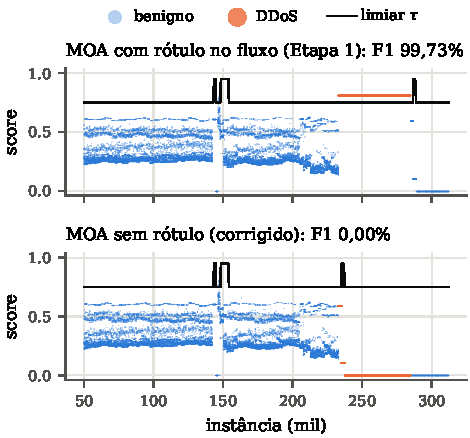
\includegraphics[width=\columnwidth]{leak_aseados}
\caption{ASEADOS, configuração do artigo, fase operacional: score do HST do MOA com o rótulo no
fluxo (acima) e sem ele (abaixo). Benignos amostrados (20 mil).}
\label{fig:leak}
\end{figure}

Normalizar os atributos e acrescentar as taxas (\modus+) não resolve. Nas três bases o \modus+ fica
com F1 abaixo de 1\% (Tabela~\ref{tab:main}), e a medida de envenenamento explica por quê: 99,96\%
dos fluxos DDoS do ASEADOS, 100,00\% dos pacotes de ataque do CTU-13 e 99,99\% dos do Edge-IIoT
treinam o modelo. A AUC-ROC do score é 17,88\%, 0,15\% e 32,87\%, respectivamente. O treino
seletivo falha em cadeia: as primeiras instâncias do ataque ficam abaixo do limiar, treinam o HST,
e as seguintes, iguais a elas, passam a ter massa na referência. No CTU-13, com $W=250$ e um
\emph{flood} de milhares de pacotes por segundo, a referência é substituída dezenas de vezes por
segundo, e o ataque passa a ser o perfil de referência em uma fração de segundo.

O \modus\ original escapa desse efeito em duas bases, mas por um motivo que não é o volume. Sem
normalização, o HST separa por protocolo (Seção~\ref{sec:replication}). No CTU-13 o \emph{flood} é
ICMP, raro no tráfego benigno, e a AUC chega a 99,86\%. No Edge-IIoT, os \emph{floods} ICMP e UDP
têm 100,00\% de alarme, enquanto os \emph{floods} TCP e HTTP têm 0,01\% e 0,02\%
(Tabela~\ref{tab:edge}). É um detector de protocolo raro: acerta quando o ataque usa um protocolo
incomum na rede e erra por completo quando usa o protocolo dominante.

\subsection{ASEADOS: ablação}
A Tabela~\ref{tab:abl} e a Figura~\ref{fig:abl} decompõem o resultado do ASEADOS. Ligadas uma a
uma sobre o \modus+, três das quatro defesas não mudam o F1, que fica abaixo de 0,4\%. O teto de
treino reduz o envenenamento de 99,96\% para 75,21\%, o que ainda é ataque suficiente para dominar
o modelo. Só o modelo congelado detecta algo sozinho (F1 de 16,18\%), e com precisão baixa
(49,30\%). O conjunto completo chega a 62,99\% de F1, com precisão de 95,19\% e 0,48\% de falsos
positivos.

\begin{table}[t]
\centering
\caption{Ablação no ASEADOS (DDoS), fase operacional (\%). ``Aquec.'': instância em que o
aquecimento termina.}
\label{tab:abl}
\setlength{\tabcolsep}{3.5pt}
\begin{tabular}{lrrrrr}
\toprule
Variante & Aquec. & Prec. & F1 & FPR & Env. \\
\midrule
\modus+ (base)             & 50.000 &  0,43 &  0,08 & 2,39 & 99,96 \\
\ + janela de 10\,s        & 50.000 &  2,00 &  0,37 & 2,42 & 99,80 \\
\ + aquecimento adaptativo &  6.651 &  0,96 &  0,05 & 0,53 & 99,97 \\
\ + teto de treino         & 50.000 &  0,67 &  0,12 & 2,38 & 75,21 \\
\ + normalização congelada & 50.000 &  0,81 &  0,15 & 2,43 & 99,92 \\
\ + modelo congelado       & 50.000 & 49,30 & 16,18 & 2,43 & 90,33 \\
\midrule
\modusp\ (todas)           &  6.651 & 95,19 & \textbf{62,99} & 0,48 & 51,24 \\
\ sem janela em tempo      &  6.651 & 93,00 & 62,45 & 0,72 & 51,30 \\
\ sem teto de treino       &  6.651 & 94,67 & 62,88 & 0,54 & 52,93 \\
\ sem aquec. adaptativo    & 50.000 & 54,39 & 19,72 & 2,47 & 74,16 \\
\ sem modelo congelado     &  6.651 &  8,15 &  0,24 & 0,28 & 65,12 \\
\bottomrule
\end{tabular}
\end{table}

\begin{figure}[t]
\centering
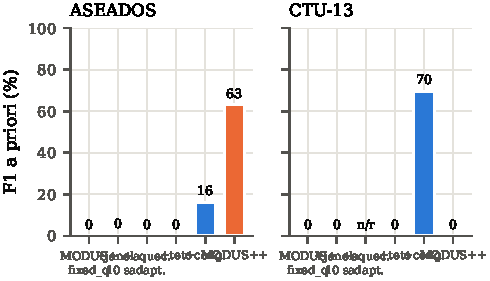
\includegraphics[width=\columnwidth]{ablation}
\caption{F1 a priori por variante. Cada barra azul liga uma defesa sobre o \modus+; a laranja é o
\modusp\ completo. No CTU-13, janela e teto foram avaliados juntos, e o aquecimento adaptativo
sozinho não foi rodado (n/r).}
\label{fig:abl}
\end{figure}

A segunda metade da tabela retira uma peça por vez do \modusp. Sem o modelo congelado o F1 volta a
0,24\%. Sem o aquecimento adaptativo cai para 19,72\%. Sem a janela em tempo ou sem o teto, quase
não muda (62,45\% e 62,88\%). O resultado no ASEADOS vem, portanto, da combinação de duas peças:
o modelo congelado e o aquecimento adaptativo.

A interação entre as duas tem explicação. Com o aquecimento fixo de 50 mil fluxos, o modelo
congelado é treinado com 40 mil e calibrado com 10 mil; o limiar resultante é $\tau_f=0{,}876$, e o
recall é 12,05\%. Com o aquecimento adaptativo, que termina em 6.651 fluxos, o congelado usa 5.320
para treino e 1.331 para calibração, o limiar é $\tau_f=0{,}818$ e o recall sobe para 47,07\%. Os
falsos positivos caem junto, de 2,47\% para 0,48\%. Esse efeito não depende do congelado: ligado
sozinho sobre o \modus+, o aquecimento adaptativo já reduz os falsos positivos de 2,39\% para
0,53\%.

A Figura~\ref{fig:frozen} mostra por que o congelado é a peça decisiva. No modelo adaptativo, a
massa dos fluxos DDoS fica à esquerda da dos benignos: o ataque foi aprendido (AUC de 27,33\%). No
modelo congelado, que nunca viu o ataque, o DDoS fica à direita, com AUC de 94,44\%. O limiar
$\tau_f$, porém, corta a distribuição do ataque ao meio. É por isso que o recall para em 47\%: a
separação existe, mas o quantil 0,999 do aquecimento não cai no vale entre as duas distribuições.

\begin{figure}[t]
\centering
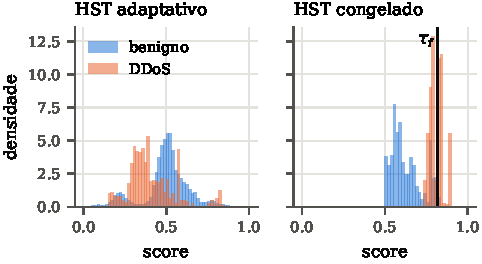
\includegraphics[width=\columnwidth]{frozen_aseados}
\caption{ASEADOS, \modusp: distribuição dos scores pós-aquecimento no HST adaptativo e no HST
congelado. A linha vertical é o limiar $\tau_f$.}
\label{fig:frozen}
\end{figure}

\textbf{Sementes.} Com três sementes do HST, o F1 do \modusp\ é 62,99\%, 68,36\% e 58,86\% (média
de 63,40\%). O \modus+ fica em 0,08\%, 0,18\% e 0,24\%. O ganho não depende da semente, mas a
variação entre sementes, de quase dez pontos, é grande: o limiar congelado vale 0,818, 0,768 e
0,865 nas três rodadas, e a semente 2 troca precisão (81,72\%) por recall (58,75\%).

\subsection{CTU-13: o envenenamento some, o limiar falha}
\label{sec:ctu}
No CTU-13 o resultado a priori do \modusp\ é negativo: F1 de 0,01\%. Os componentes, vistos em
separado, mostram que o método faz o que foi projetado para fazer, e que o erro está em um ponto
específico (Tabela~\ref{tab:ctu} e Figura~\ref{fig:ctu}).

\begin{table}[t]
\centering
\caption{CTU-13, cenário 11, fase operacional (\%). AUC do score do modelo adaptativo. As duas
últimas linhas são análise de sensibilidade, não resultado a priori.}
\label{tab:ctu}
\setlength{\tabcolsep}{3.5pt}
\begin{tabular}{lrrrr}
\toprule
Variante & F1 & FPR & Env. & AUC \\
\midrule
\modus+ (base)              &  0,00 & 3,12 & 100,00 &  0,15 \\
\ + modelo congelado        & 69,59 & 2,73 &  43,58 & 49,78 \\
\ + janela de 10\,s e teto  &  0,00 & 0,04 &   2,07 & 96,47 \\
\modusp\ (todas)            &  0,01 & 2,60 &   2,41 & 72,93 \\
\midrule
\modusp, teto $0{,}1\,c$    & 88,26 & 9,21 &   0,05 & 90,41 \\
\modusp, quantil 0,99       & 83,40 & 5,01 &   0,89 & 92,71 \\
\bottomrule
\end{tabular}
\end{table}

\begin{figure}[t]
\centering
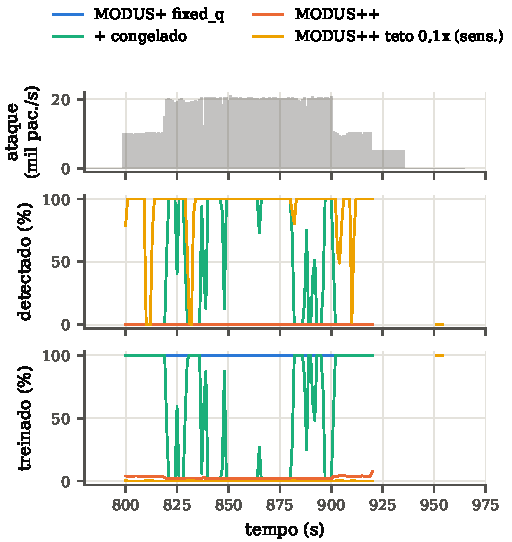
\includegraphics[width=\columnwidth]{ctu_timeline}
\caption{CTU-13, intervalo do \emph{flood}. Acima: pacotes de ataque por segundo. No meio: fração
do ataque detectada. Abaixo: fração do ataque usada no treino do modelo adaptativo.}
\label{fig:ctu}
\end{figure}

\textbf{Janela em tempo e teto eliminam o envenenamento.} Com as duas defesas, a fração do
\emph{flood} que entra no treino cai de 100,00\% para 2,07\%, e a AUC do score adaptativo sobe de
0,15\% para 96,47\%. O teto calculado no aquecimento é de 342 instâncias por segundo por destino,
contra um ataque de 10 a 20 mil pacotes por segundo sobre um único alvo. O modelo deixa de aprender
o ataque e volta a pontuá-lo como anômalo. O F1, porém, continua em 0,00\%, porque o limiar
adaptativo não acompanha: com um limiar fixo escolhido com rótulos, o mesmo score daria F1 de
94,81\%. Esse valor é um teto, não um resultado.

\textbf{O congelado sozinho detecta, mas não protege.} Ligado sobre o \modus+, sem as outras
defesas, o modelo congelado chega a 69,59\% de F1, com precisão de 90,79\% e recall de 56,42\%. A
Figura~\ref{fig:ctu} mostra que a detecção oscila: nos segundos em que o score congelado fica abaixo
de $\tau_f$, o ataque volta a treinar o modelo adaptativo, e 43,58\% do \emph{flood} é aprendido.

\textbf{No conjunto completo, o limiar erra por milésimos.} No \modusp\ o aquecimento adaptativo
termina em 35.318 pacotes, e o congelado é calibrado com $\tau_f=0{,}777$. O score do \emph{flood}
nesse modelo é 0,774. O ataque fica logo abaixo do limiar durante todo o intervalo, e a linha
laranja da Figura~\ref{fig:ctu} não sai do zero. A AUC do congelado é 93,95\%: a separação existe,
como no ASEADOS, e o limiar não a aproveita. As duas rodadas de sensibilidade confirmam a leitura.
Com o quantil 0,99 em vez de 0,999, $\tau_f$ cai para 0,734 e o F1 vai a 83,40\%. Com o teto
dividido por dez, o F1 vai a 88,26\%, ao custo de 9,21\% de falsos positivos. Nenhum dos dois
valores foi escolhido a priori, e não os contamos como resultado do método.

Vale registrar a comparação desfavorável: o \modus\ original, sem normalização, tem F1 de 64,55\%
nesta base com os hiperparâmetros do artigo e de 99,74\% com os hiperparâmetros que o artigo usa no
ASEADOS. Os dois valores vêm da raridade do ICMP, e a diferença entre eles ilustra o peso do
ajuste por base: com a configuração do artigo para o CTU-13, 52,37\% do tráfego benigno gera alarme.

\subsection{Edge-IIoTset e ataques não-DDoS}
\label{sec:edge}
No Edge-IIoTset usamos os 14 tipos de ataque da base (21,1 milhões de quadros, 9,87 milhões de
ataque). É o melhor resultado do \modusp: F1 de 91,17\%, com precisão de 96,03\% e recall de
86,77\%, contra 76,66\% do \modus\ original e 0,01\% do \modus+. O envenenamento cai de 99,99\%
para 6,90\%, e a AUC do score adaptativo vai de 32,87\% para 91,95\%. O aquecimento adaptativo
termina no mínimo permitido, 5.000 quadros.

\begin{table}[t]
\centering
\caption{Edge-IIoTset: taxa de alarme por classe na fase operacional (\%). $n$ em milhares de
quadros (no \modusp, 11.254 mil normais, pois o aquecimento é mais curto).}
\label{tab:edge}
\setlength{\tabcolsep}{4pt}
\begin{tabular}{lrrrr}
\toprule
Classe & $n$ & \modus & \modus+ & \modusp \\
\midrule
DDoS ICMP             &  2.914 & 100,00 & 0,00 & 99,88 \\
DDoS UDP              &  3.216 & 100,00 & 0,00 & 99,72 \\
DDoS TCP              &  2.020 &   0,01 & 0,00 & 97,14 \\
DDoS HTTP             &    229 &   0,02 & 0,05 & 68,32 \\
\midrule
Vulnerability scanner &    266 &   0,13 & 0,09 & 77,75 \\
Ransomware            &     11 &  11,19 & 0,08 & 43,30 \\
Fingerprinting        &      1 &  69,22 & 0,00 & 34,86 \\
MITM                  &      1 &  66,80 & 3,91 & 18,31 \\
SQL injection         &     51 &   0,11 & 0,00 & 16,45 \\
Backdoor              &     25 &   3,32 & 0,01 & 12,92 \\
Password              &  1.054 &   0,17 & 0,00 &  9,05 \\
Uploading             &     38 &   0,16 & 0,06 &  8,25 \\
Port scanning         &     23 &  11,40 & 0,05 &  5,88 \\
XSS                   &     16 &   4,55 & 0,00 &  4,30 \\
\midrule
Normal (falso alarme) & 11.209 &   0,12 & 0,01 &  3,14 \\
\bottomrule
\end{tabular}
\end{table}

A Tabela~\ref{tab:edge} detalha por classe. O ganho sobre o \modus\ original está nos
\emph{floods} que usam o protocolo dominante da rede: o DDoS TCP vai de 0,01\% para 97,14\% de
alarme, e o DDoS HTTP, de 0,02\% para 68,32\%. Os \emph{floods} ICMP e UDP continuam acima de
99,7\%. O custo é o falso alarme no tráfego normal, que sobe de 0,12\% para 3,14\%.

Fora dos DDoS, o resultado é fraco. Só o \emph{Vulnerability scanner} passa de 50\% de alarme. Sete
das dez classes não-DDoS ficam abaixo de 20\%, e \emph{Password}, a mais volumosa delas, tem
9,05\%, pouco acima da taxa de falso alarme. Em quatro classes pequenas (\emph{Fingerprinting},
MITM, \emph{Port scanning} e XSS), o \modus\ original tem taxa maior que a do \modusp. Os atributos usados (portas, protocolo,
tamanho e taxas) descrevem volume e cabeçalho, e não o conteúdo que caracteriza esses ataques. O
F1 alto no Edge-IIoT vem dos DDoS, que são 85\% das instâncias de ataque.

O ASEADOS com as cinco classes mostra o outro lado do modelo congelado. O \modusp\ sobe de 0,71\%
para 31,15\% de F1 e detecta 100,00\% do \emph{Probe}, mas apenas 38,82\% do DDoS, 22,90\% do
\emph{Bot} e 10,95\% do DoS, com 17,88\% de falsos positivos. Nessa variante há ataques
desde o início do fluxo: os primeiros 50 mil fluxos contêm 20.711 deles. O modelo congelado
depende de um aquecimento limpo, e a AUC do seu score aqui é 50,05\%, igual ao acaso.

\subsection{Sensibilidade}
\label{sec:sens}
Os parâmetros novos foram fixados antes das rodadas. Variamos três deles depois, para medir o quanto
o resultado depende dessas escolhas (Tabela~\ref{tab:sens}).

\begin{table}[t]
\centering
\caption{Sensibilidade do \modusp\ aos parâmetros novos (\%). A primeira linha de cada base é a
configuração a priori.}
\label{tab:sens}
\setlength{\tabcolsep}{3pt}
\begin{tabular}{llrrrr}
\toprule
Base & Variação & Prec. & Rec. & F1 & FPR \\
\midrule
\multirow{4}{*}{ASEADOS}
 & a priori ($T=10$\,s; $q=0{,}999$) & 95,19 & 47,07 & 62,99 & 0,48 \\
 & $T=1$\,s        & 99,01 &  9,88 & 17,97 & 0,02 \\
 & $T=60$\,s       & 93,85 & 47,19 & 62,80 & 0,63 \\
 & $q=0{,}99$      & 81,69 & 48,83 & 61,12 & 2,22 \\
\midrule
\multirow{3}{*}{CTU-13}
 & a priori ($c$; $q=0{,}999$)       &  0,06 &  0,00 &  0,01 & 2,60 \\
 & teto $0{,}1\,c$ & 82,96 & 94,29 & 88,26 & 9,21 \\
 & $q=0{,}99$      & 88,24 & 79,07 & 83,40 & 5,01 \\
\bottomrule
\end{tabular}
\end{table}

No ASEADOS o método é estável para janelas de 10 e 60 segundos e para o quantil do limiar
congelado. A janela de 1 segundo degrada o resultado (F1 de 17,97\%): com ela o aquecimento
adaptativo termina em outro ponto (12.025 fluxos), o limiar congelado sobe para $\tau_f=0{,}854$ e
o recall cai para 9,88\%. Uma explicação provável é que, na taxa baixa desta base, janelas de
1 segundo raramente juntam as 50 instâncias exigidas para a troca. No CTU-13 a sensibilidade é extrema, pelo motivo já visto: qualquer variação que
mova o limiar ou o score em poucos milésimos leva o F1 de 0\% para mais de 80\%. Um resultado que
muda tanto com uma casa decimal de um quantil não deve ser lido nem como fracasso nem como sucesso
do modelo, e sim como evidência de que a regra de limiar é o elo fraco.

\subsection{Custo computacional}
O \modusp\ mantém dois HST e pontua cada instância nos dois. Ainda assim o motor em \texttt{numpy}
processou o CTU-13 (6,3 milhões de pacotes) em 1.294\,s e o Edge-IIoTset (21,1 milhões de quadros)
em 1.384\,s, cerca de 4,9 mil e 15,3 mil instâncias por segundo. O ganho vem do cálculo em lote: o
score de uma janela inteira é calculado de uma vez, porque a referência não muda entre trocas. Os
tempos são indicativos, pois várias rodadas dividiram a mesma máquina. Para o mesmo fluxo do
Edge-IIoTset, o artigo original reporta 14.893\,s.

\section{Discussão}
\label{sec:discussion}

\subsection{O que a replicação mostra sobre o \modus}
A replicação separa três afirmações que o artigo original apresenta juntas. A primeira é que o
método atinge os F1 reportados. Isso se reproduz em duas das três bases, mas no ASEADOS só com o
rótulo no fluxo, e no Edge-IIoTset com VP e FN idênticos em um conjunto que conta o tráfego normal
duas vezes. A segunda é que a detecção é volumétrica. Não é: sem normalização, o HST responde à
raridade do protocolo, e o recall de 73,16\% no Edge-IIoTset é exatamente a fração de pacotes DDoS
que não são TCP. A terceira é que a \emph{flag} de mudança de conceito informa o detector. Ela muda
um pacote em 19,6 milhões.

Não afirmamos que os autores usaram o rótulo. O código não é público, e o texto não diz como o
fluxo foi montado. O que os dados sustentam é mais restrito: com o HST do MOA e o uso padrão do
CapyMOA, o rótulo chega ao detector, e o número do ASEADOS se reproduz com ele e não se
reproduz sem ele. A coincidência justifica pedir aos autores a publicação do código.

\subsection{Um vazamento que a API não mostra}
O vazamento descrito na Seção~\ref{sec:leak} não exige erro do usuário. O \texttt{NumpyStream} do
CapyMOA recebe \texttt{X} e \texttt{y}, como qualquer fluxo de avaliação, e o \texttt{HSTrees}
aparece na biblioteca como detector de anomalia de uma classe. Nada na interface indica que o
atributo de classe entra nas dimensões de corte. O efeito também não é uniforme, e isso o torna
difícil de notar: no CTU-13 as predições com e sem rótulo são idênticas, porque os atributos já
separam as classes. Um teste em uma só base poderia concluir que não há problema.

Duas verificações simples teriam revelado o defeito, e as recomendamos para qualquer avaliação de
detector não supervisionado: (i) repetir a rodada com rótulos constantes ou embaralhados, pois o
resultado não pode mudar; (ii) pontuar o mesmo vetor de atributos com rótulos diferentes. Ambas se
enquadram no que Arp \emph{et al.}~\cite{arp2022dos} chamam de checagem de \emph{label leakage}, e
custam uma rodada a mais.

\subsection{Envenenamento sem adversário}
A literatura de envenenamento costuma supor um atacante que conhece o detector e injeta tráfego
aos poucos~\cite{rubinstein2009antidote}. Nossos resultados mostram um caso mais simples e mais
comum: o próprio ataque volumétrico, sem nenhuma intenção de evasão, envenena o modelo. Bastam
duas condições, ambas presentes no \modus: o detector treina com o que classifica como benigno, e
o ritmo de atualização do modelo é medido em instâncias. Um \emph{flood} produz instâncias na
taxa que quiser; logo, controla o relógio do modelo.

Daí a utilidade de reportar a fração do ataque usada no treino. O F1 diz se o detector acertou; a
fração treinada diz se ele continuará acertando. No CTU-13, por exemplo, o modelo congelado
sozinho tem o melhor F1 a priori (69,59\%), mas 43,58\% do \emph{flood} treina o modelo adaptativo.
Já a combinação de janela em tempo e teto tem F1 nulo e um modelo íntegro, com AUC de 96,47\%. Só
o F1 esconderia essa diferença.

\subsection{O papel de cada defesa}
As quatro defesas agem em pontos diferentes, e as bases as exercitam de modo diferente. A janela em
tempo e o teto limitam a \emph{velocidade} com que o ataque entra no modelo. São decisivos no
CTU-13, onde o ataque chega a 20 mil pacotes por segundo, e quase irrelevantes no ASEADOS, onde o
DDoS tem cerca de 46 fluxos por segundo e o teto de 24,9 por destino quase não atua: com e sem
ele, o envenenamento é de 51,24\% e 52,93\%. O modelo congelado age sobre a \emph{decisão}: ele mantém uma referência que o ataque não
alcança. É decisivo no ASEADOS e necessário em todas as bases, pois sem ele o limiar adaptativo
não dispara mesmo quando o score separa bem as classes. O aquecimento adaptativo decide \emph{com
que dados} o congelado é construído, e seu efeito no ASEADOS foi maior do que esperávamos.

O modelo congelado tem um custo conhecido, e os dados o confirmam. Ele pressupõe aquecimento limpo:
no ASEADOS com cinco classes, em que há ataques desde o início do fluxo, sua AUC é 50,05\%. E ele não
acompanha a deriva do tráfego legítimo: os falsos positivos sobem para 3,14\% no Edge-IIoTset e
17,88\% no ASEADOS com cinco classes. Em operação real, um modelo congelado precisaria ser refeito
periodicamente, em janelas validadas como limpas, o que reintroduz alguma supervisão.

\subsection{O limiar é o gargalo}
O resultado mais consistente entre as bases é a distância entre separabilidade e decisão. No
ASEADOS o score congelado tem AUC de 94,44\% e o recall é 47,07\%. No CTU-13 a AUC é 93,95\% e o
recall é 0,00\%. Nos dois casos o modelo ordena bem as instâncias, e a regra de limiar, um quantil
alto dos scores do aquecimento, corta no lugar errado. Um quantil estima a cauda do tráfego
\emph{benigno}; ele nada diz sobre onde o ataque vai cair. Com 1.331 a 7.064 instâncias de
calibração, o quantil 0,999 é determinado por uma a sete observações, o que também explica a
variação de $\tau_f$ entre sementes.

Vemos três caminhos, todos sem rótulos: (i) decidir por janela, e não por instância, exigindo que
uma fração dos scores de um destino passe de um quantil mais baixo, o que explora a persistência do
\emph{flood}; (ii) combinar os scores dos dois modelos em vez de fazer um \emph{ou} lógico entre
dois limiares; (iii) calibrar o limiar com a teoria de valores extremos sobre a cauda do
aquecimento, em vez de um quantil empírico. Não testamos nenhum deles.

\subsection{Ameaças à validade}
\textbf{Ordem do ASEADOS.} A ordem ``temporal'' que usamos é a que reproduz o artigo, e ela vem de
uma leitura errada das datas. Na ordem cronológica correta, o DDoS ocupa os primeiros 50 mil
fluxos, e nenhum método que aprende o normal no início do fluxo pode detectá-lo. Os resultados do
ASEADOS valem para a ordem do artigo, não para a base como foi coletada.

\textbf{Rótulos por pacote.} No CTU-13 o rótulo vem do IP infectado, e no Edge-IIoTset, do arquivo
de captura. Pacotes legítimos de uma máquina infectada, ou tráfego de fundo dentro de um
\emph{pcap} de ataque, contam como ataque. Isso limita o recall alcançável e afeta todos os métodos
igualmente.

\textbf{Uma rodada por base.} Só o ASEADOS foi rodado com três sementes. No CTU-13 e no
Edge-IIoTset há uma rodada por configuração. Dada a variação de dez pontos entre sementes no
ASEADOS, diferenças pequenas entre variantes não devem ser interpretadas.

\textbf{Parâmetros a priori.} A configuração \texttt{fixed\_q} e os parâmetros novos foram fixados
antes das rodadas da Etapa~2, mas por nós, que já conhecíamos as bases da Etapa~1. As rodadas de
sensibilidade estão identificadas como tal, e o resultado negativo do CTU-13 foi mantido como
resultado principal para não esconder essa dependência.

\textbf{Bases de laboratório.} As três bases têm ataques longos, intensos e de vetor único, depois
de um período benigno. Ataques curtos, de baixa taxa ou presentes desde o início não estão
representados.

\section{Conclusão}
\label{sec:conclusion}

Replicamos o \modus\ a partir do texto do artigo e implementamos as melhorias propostas na primeira
etapa do trabalho. O percurso produziu três resultados.

O primeiro é um defeito de avaliação. O \texttt{HSTrees} do MOA usa o atributo de classe como
dimensão de corte, e o uso padrão do CapyMOA entrega o rótulo verdadeiro ao detector. No
ASEADOS-SDN-IoT, o F1 de 99,73\% da nossa réplica cai para 0,00\% quando o rótulo sai do fluxo. O
efeito depende da base, o que o torna fácil de não ver.

O segundo é um defeito de projeto. Sem o vazamento, o treino seletivo do \modus\ e da sua versão
normalizada deixa de 99,96\% a 100\% do ataque entrar no modelo nas três bases. O \emph{flood}
vira o perfil normal, e a AUC do score fica abaixo de 50\%. Onde o \modus\ original ainda detecta,
é pela raridade do protocolo do ataque, e não pelo volume.

O terceiro é o \modusp, com quatro defesas causais e sem rótulos. Com uma única configuração, o F1
vai de 0,08\% para 62,99\% no ASEADOS e de 76,66\% para 91,17\% no Edge-IIoTset, onde o método
passa a detectar os \emph{floods} TCP e HTTP que o original perdia. No CTU-13 as defesas reduzem o
envenenamento de 100\% para 2,41\%, mas o F1 a priori é 0,01\%, porque o score do ataque fica
milésimos abaixo do limiar. Ataques não-DDoS continuam, em sua maioria, sem detecção.

As limitações apontam os próximos passos. A calibração do limiar sem rótulos é a principal: nas
duas bases em que medimos, o modelo congelado separa as classes com AUC de 94\% e a regra de quantil
desperdiça a separação. A decisão por janela e por destino é o caminho que consideramos mais
promissor. Faltam ainda a renovação periódica do modelo congelado, a avaliação com mais sementes
nas bases grandes e bases com ataques curtos ou de baixa taxa.

Para quem avalia detectores de anomalia em fluxos, ficam três recomendações práticas: verificar
que o resultado não muda com rótulos constantes; reportar a fração do ataque usada no treino, e
não só o F1; e fixar uma configuração única para todas as bases antes de olhar os resultados. O
código, os \emph{logs} e as métricas de todas as rodadas estão no repositório do trabalho.


\bibliographystyle{IEEEtran}
\bibliography{refs}

\end{document}
